% !TeX TXS-program:compile = txs:///lualatex/[--shell-escape]

%----------------------- Преамбула -----------------------
\documentclass[ut8x, 14pt, oneside, a4paper]{extarticle}

\usepackage{extsizes} % Для добавления в параметры класса документа 14pt

% Для работы с несколькими языками и шрифтом Times New Roman по-умолчанию
\usepackage[english,russian]{babel}
\usepackage{fontspec}
\setmainfont{Times New Roman}
\usepackage[left=30mm,right=10mm,top=20mm,bottom=20mm]{geometry}
\usepackage{misccorr}
\usepackage{indentfirst}
\usepackage{enumitem}
\usepackage{pdfpages}
%\usepackage{ragged2e}
\setlength{\parindent}{1.25cm}
%\setlength{\parskip}{1em} % поменять
%\linespread{1.3}
\renewcommand{\baselinestretch}{1.5}
\setlist{nolistsep} % Отсутствие отступов между элементами \enumerate и \itemize

% Дополнительное окружения для подписей
\usepackage{array}
\newenvironment{signstabular}[1][1]{
	\renewcommand*{\arraystretch}{#1}
	\tabular
}{
	\endtabular
}

% Переопределение стандартных \section, \subsection, \subsubsection по ГОСТу;
% Переопределение их отступов до и после для 1.5 интервала во всем документе
\usepackage{titlesec}

\titleformat{\section}[block]
{\bfseries\normalsize\filcenter}{\thesection}{1em}{}

\titleformat{\subsection}[hang]
{\bfseries\normalsize}{\thesubsection}{1em}{}
\titlespacing\subsection{\parindent}{\parskip}{\parskip}

\titleformat{\subsubsection}[hang]
{\bfseries\normalsize}{\thesubsubsection}{1em}{}
\titlespacing\subsubsection{\parindent}{\parskip}{\parskip}

\newcommand{\specsection}[1]{\section*{#1}\addcontentsline{toc}{section}{#1}}

% Работа с изображениями и таблицами; переопределение названий по ГОСТу
\usepackage{caption}
\captionsetup[figure]{name={Рисунок},labelsep=endash}
\captionsetup[table]{singlelinecheck=false, labelsep=endash}

\usepackage{graphicx}
\usepackage{diagbox} % Диагональное разделение первой ячейки в таблицах

% Цвета для гиперссылок и листингов
\usepackage{color}

% Гиперссылки \toc с кликабельностью
\usepackage[linktoc=all]{hyperref}
\hypersetup{hidelinks}

% Листинги
%\setsansfont{Arial}
%\setmonofont{Courier New}

\usepackage{color} % Цвета для гиперссылок и листингов
%\definecolor{comment}{rgb}{0,0.5,0}
%\definecolor{plain}{rgb}{0.2,0.2,0.2}
%\definecolor{string}{rgb}{0.91,0.45,0.32}
%\hypersetup{citecolor=blue}
\hypersetup{citecolor=black}

\usepackage{listings}
\lstset{
	basicstyle=\footnotesize\ttfamily,
	language=XML, % Или другой ваш язык -- см. документацию пакета
	commentstyle=\color{comment},
	numbers=left,
	numberstyle=\tiny,
	numbersep=5pt,
	tabsize=4,
	extendedchars=\true,
	breaklines=true,
	keywordstyle=\color{blue},
	frame=b,
	stringstyle=\ttfamily\color{string}\ttfamily,
	showspaces=false,
	showtabs=false,
	xleftmargin=17pt,
	framexleftmargin=17pt,
	framexrightmargin=5pt,
	framexbottommargin=4pt,
	showstringspaces=false,
	inputencoding=utf8x,
	keepspaces=true
}

\DeclareCaptionLabelSeparator{line}{\ --\ }
\DeclareCaptionFont{white}{\color{white}}
\DeclareCaptionFormat{listing}{\colorbox[cmyk]{0.43,0.35,0.35,0.01}{\parbox{\textwidth}{\hspace{15pt}#1#2#3}}}
\captionsetup[lstlisting]{
	format=listing,
	labelfont=white,
	textfont=white,
	singlelinecheck=false,
	margin=0pt,
	font={bf,footnotesize},
	labelsep=line
}

\usepackage{ulem} % Нормальное нижнее подчеркивание
\usepackage{hhline} % Двойная горизонтальная линия в таблицах
\usepackage[figure,table]{totalcount} % Подсчет изображений, таблиц
\usepackage{rotating} % Поворот изображения вместе с названием
\usepackage{lastpage} % Для подсчета числа страниц

\makeatletter
\renewcommand\@biblabel[1]{#1.}
\makeatother

\usepackage{color}
\usepackage[cache=false, newfloat]{minted}
\newenvironment{code}{\captionsetup{type=listing}}{}
\SetupFloatingEnvironment{listing}{name=Листинг}

\usepackage{amsmath}
\usepackage{slashbox}


\begin{document}
	
\begin{titlepage}
	\noindent\begin{minipage}{0.05\textwidth}
		
\includegraphics[scale=0.3]{inc/bmstu.png}
	\end{minipage}
	\hfill
	\begin{minipage}{0.85\textwidth}\raggedleft
		\begin{center}
			\fontsize{12pt}{0.3\baselineskip}\selectfont \textbf{Министерство науки и высшего образования Российской Федерации \\ Федеральное государственное бюджетное образовательное учреждение \\ высшего образования \\ <<Московский государственный технический университет \\ имени Н.Э. Баумана \\ (национальный исследовательский университет)>> \\ (МГТУ им. Н.Э. Баумана)}
		\end{center}
	\end{minipage}
	\vspace*{-0.3cm}
	\begin{center}
		\fontsize{12pt}{0.1\baselineskip}\selectfont
		\noindent\makebox[\linewidth]{\rule{\textwidth}{1pt}} \makebox[\linewidth]{\rule{\textwidth}{4pt}}
	\end{center}
	\vspace*{-1.5cm}
	\begin{flushleft}
		\fontsize{12pt}{\baselineskip}\selectfont 
		
		ФАКУЛЬТЕТ ИУ <<Информатика и системы управления>>

		КАФЕДРА ИУ-7 <<Программное обеспечение ЭВМ и информационные технологии>>
	\end{flushleft}

	\vfill

	\begin{center}
		\fontsize{20pt}{\baselineskip}\selectfont

		\textbf{РАСЧЕТНО-ПОЯСНИТЕЛЬНАЯ ЗАПИСКА}

		\textbf{\textit{К НАУЧНО-ИССЛЕДОВАТЕЛЬСКОЙ РАБОТЕ}}

		\textbf{\textit{НА ТЕМУ:}}
	\end{center}

	\begin{center}
		\fontsize{20pt}{0.6cm}\selectfont 
		
		\textit{\bfseries{<<Применение сетей Петри для моделирования цифрового документооборота>>}}
		
	\end{center}

	\vfill
	
	\fontsize{12pt}{0.6cm}\selectfont
	Студент \hspace{1.1cm} ИУ7-75Б \hspace{3.83cm} \uline{\mbox{\hspace*{3.5cm}}}~ \textbf{Богаченко А. Е.}
	
	\vfill
	
	Руководитель НИР \hspace{4.8cm} \uline{\mbox{\hspace*{3.5cm}}}~ \textbf{Строганов Ю. В.}
	
	~~
	
	\textit{Рекомендуемая руководителем НИР оценка}~\uline{\mbox{\hspace*{3.5cm}}}
	
	\vfill

	\begin{center}
		\normalsize \textit{\the \year~г.}
	\end{center}
\end{titlepage}
\pagenumbering{gobble}
\setlength\parindent{0pt}
\begin{center}
	\fontsize{12pt}{0.3\baselineskip}\selectfont \textbf{Министерство науки и высшего образования Российской Федерации \\ Федеральное государственное бюджетное образовательное учреждение \\ высшего образования \\ <<Московский государственный технический университет имени Н.Э. Баумана \\ (национальный исследовательский университет)>> \\ (МГТУ им. Н.Э. Баумана)}
\end{center}
\vspace*{-0.5cm}
\begin{center}
	\fontsize{12pt}{0.1\baselineskip}\selectfont
	\noindent\makebox[\linewidth]{\rule{\textwidth}{1pt}} \makebox[\linewidth]{\rule{\textwidth}{4pt}}
\end{center}

\begin{flushright}
	\fontsize{12pt}{0.4cm}\selectfont
	УТВЕРЖДАЮ\mbox{\hspace{2.5cm}}
	
	Заведующий кафедрой ИУ-7
	
	\uline{\mbox{\hspace{3cm}}} И. В. Рудаков
	
	<<16>> сентября 2023г.
\end{flushright}

\begin{center}
	\fontsize{20pt}{14pt}\selectfont

	\textbf{З А Д А Н И Е}
	
	\textbf{на выполнение научно-исследовательской работы}
\end{center}


\fontsize{12pt}{0.6cm}\selectfont	

по теме 
	
\makebox[\linewidth]{\textbf{<<Применение сетей Петри для моделирования цифрового документооборота>>}}
	
Студент группы \textbf{ИУ7-75Б}
	
\makebox[\linewidth]{\textbf{Богаченко Артём Евгеньевич}}
	
Направленность НИР
	
\makebox[\linewidth]{\textbf{учебная}}
	
Источник тематики
	
\makebox[\linewidth]{\textbf{НИР кафедры}}
	
График выполнения НИР: ~25\% к 6 нед., 50\% к 9 нед., 75\% к 12 нед., 100\% к 15 нед.
	
~~
	
\textit{\bfseries{Техническое задание}}

\textit{Провести обзор существующих методов моделирования цифрового документооборота. Провести анализ возможности применения сетей Петри для моделирования цифрового документооборота.}
	
~~
	
\textit{\bfseries{Оформление научно-исследовательской работы:}}

Расчетно-пояснительная записка на \textbf{12-20} листах формата А4.

\textit{\bfseries{Перечень графического (иллюстративного) материала:}}	

Презентация на \textbf{6-10} слайдах.

Дата выдачи задания <<16>> сентября 2023 г.	

~~

\textbf{Руководитель НИР} \hspace{3.6cm} \uline{\mbox{\hspace*{3.5cm}}} \hspace{1.1cm} \textbf{Строганов Ю. В.}

\hfill (Подпись, дата) \hspace{1.9cm} (Фамилия И. О) \hspace{1.2cm}

\textbf{Студент} \hspace{5.7cm} \uline{\mbox{\hspace*{3.5cm}}} \hspace{1.1cm} \textbf{Богаченко А. Е.}

\hfill (Подпись, дата) \hspace{1.9cm} (Фамилия И. О) \hspace{1.2cm}
	
\setlength{\parindent}{1.25cm}

\normalsize

\pagenumbering{arabic}
\setcounter{page}{2}

\tableofcontents
\normalsize

\pagebreak

\specsection{ВВЕДЕНИЕ}

Процесс обучения -- важный этап в развитии профессиональных качеств личности. Качество методов обучения, структурированность изложения материала, а также уровень вовлечённости обучаемого напрямую влияет на предполагаемый успех и усвоение учебного материала\cite{effective-learning}. Так же на качество обучения влияет заимствование чужих работ\cite{plagiat}.

Для организации учебного процесса существует множество интерактивных систем управления обучением (англ. Learning Managment System (LMS\cite{lms})), которые облегчают процесс обучения и повышают вовлечённость обучаемого.

Цель работы -- провести обзор существующих решений в области систем управления обучением и исследовать возможности по расширению их функционала для проверки работ на предмет заимствования и корректность выполнения поставленной задачи. Правильно выполненная работа заключается в построении блок-схемы некоторого алгоритма.

Для достижения этой цели требуется решить следующие задачи НИР:
\begin{enumerate}
	\item провести обзор существующих решений в области систем управления обучением;
	\item провести обзор существующих решений в области алгоритмов поиска заимствований.
\end{enumerate}

\clearpage

\section{Анализ предметной области}
\subsection{Базовые понятия}

\subsubsection{Алгоритм}

Алгоритм -- конечная последовательность детерминированных арифметических и логических действий над исходными и промежуточными данными, выполнение которых приводит к получению требуемых выходных данных\cite{algorithms}.

\subsubsection{Схема алгоритма}

Схема алгоритма\cite{algorithms} -- один из способов визуального представления алгоритмов, ориентированный  граф,  указывающий  порядок  исполнения  команд  алгоритма. Для  описания  схем  существовало  несколько  стандартов,  из  которых  наиболее актуальным является ГОСТ 19.701-90\cite{gost}, утверждённый 01 января 1992 г. Часть описанных в стандарте символов можно увидеть на 

\noindent рисунке \ref{fig:block-scheme}.~

\begin{figure}[h!btp]
	\centering
	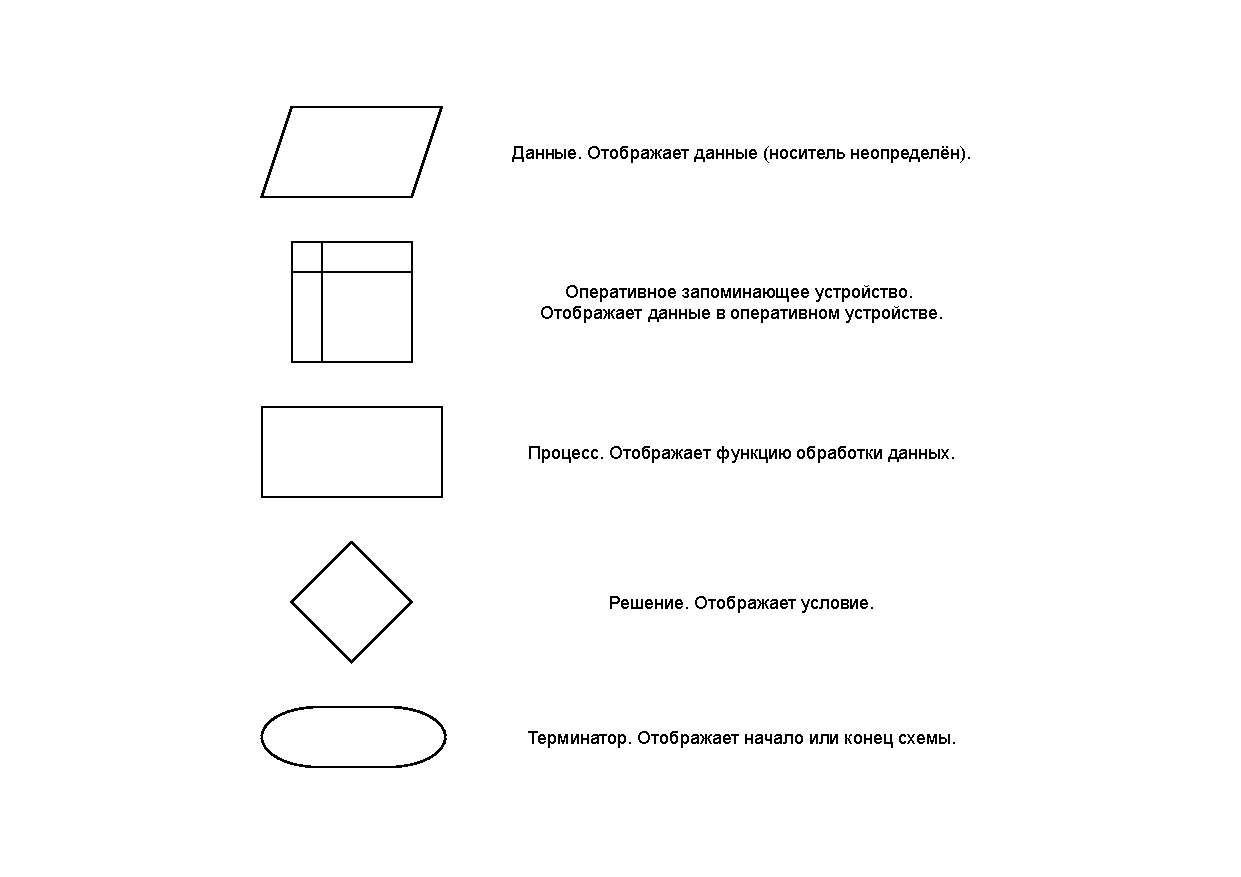
\includegraphics[width=450pt]{inc/block-scheme.pdf}
	\caption{Символы описания схемы алгоритма}
	\label{fig:block-scheme}	
\end{figure}

\clearpage

Пример реализации алгоритма вычисления суммы \textit{n} чисел представлен на рисунке \ref{fig:sum-n-scheme}.

\begin{figure}[h!btp]
	\centering
	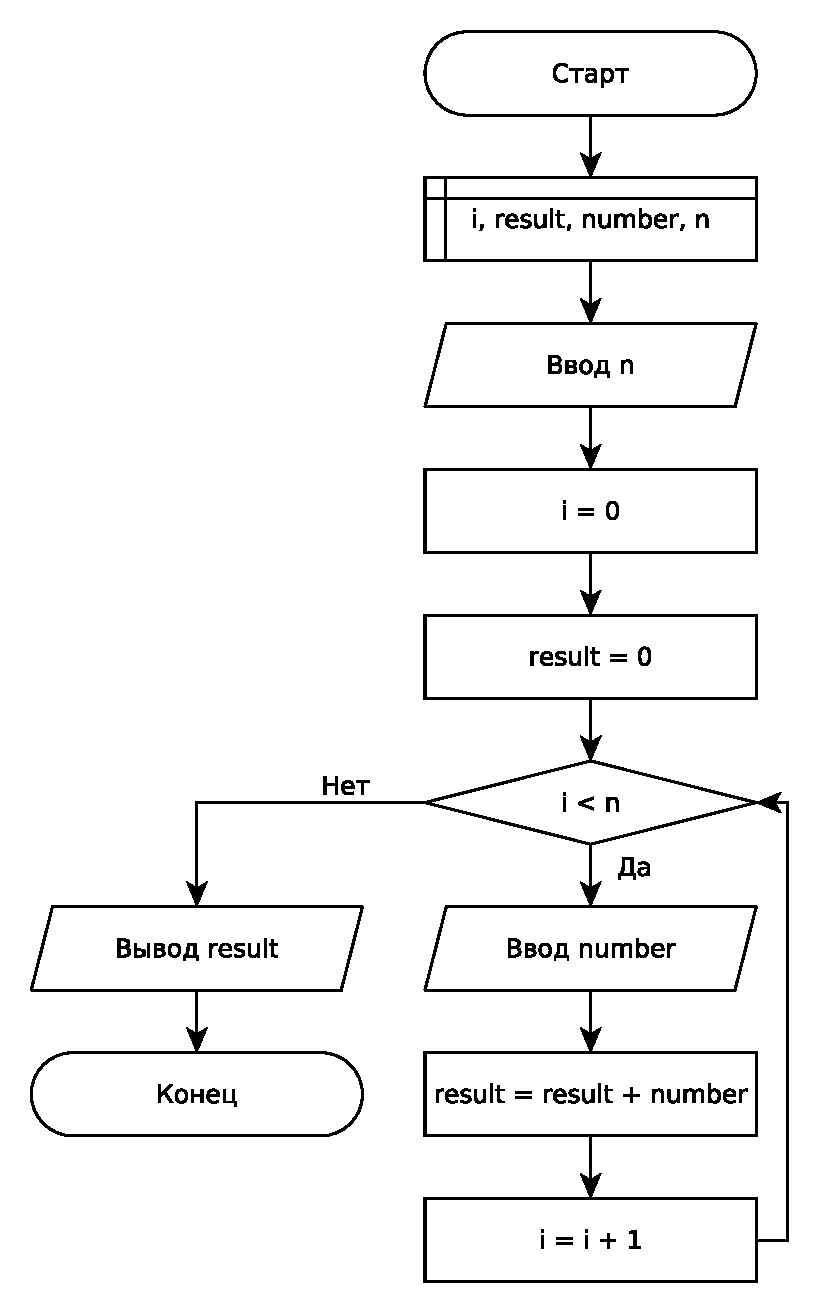
\includegraphics[width=380pt]{inc/sum-n-scheme.pdf}
	\caption{Блок-схема алгоритма вычисления суммы \textit{n} чисел}
	\label{fig:sum-n-scheme}	
\end{figure}

\clearpage

\subsubsection{Плагиат}

В общем случае плагиат -- акт заимствования (использования) слов или идей другого человека без прямого упоминания первоисточника\cite{thesaurus}. В терминах компьютерного программирования плагиатом является заимствование программной или графической (схема) реализации алгоритма.

\subsubsection{Система управления обучением}

Система управления обучением -- веб-технология, обеспечивающая поддержку преподавателей в организации процесса обучения, организации содержания курса и поддержке студентов в процессе их обучения\cite{lms-conference}. 

Пример организации интегрированной в экосистему ВУЗ-а \textit{LMS} можно увидеть на рисунке \ref{fig:LMS}.

\begin{figure}[h!btp]
	\centering
	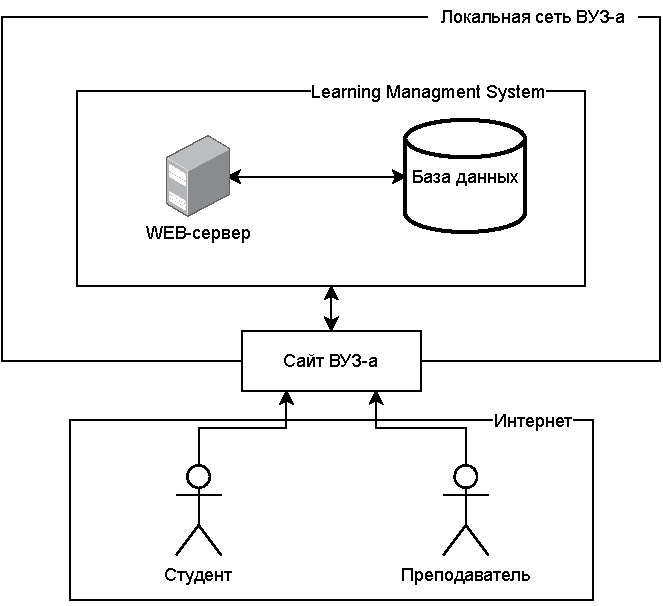
\includegraphics[width=420pt]{inc/LMS.pdf}
	\caption{Общая схема организации \textit{LMS} ВУЗ-а}
	\label{fig:LMS}	
\end{figure}

\clearpage

\section{Существующие решения}

\subsection{Системы управления обучением}

Ниже будут рассмотрены системы управления обучением в академическом домене.

\subsubsection{Moodle}

Moodle\cite{moodle} -- бесплатная система управления обучением с открытым исходным кодом. Обладает широким спектром возможностей в области организации процесса обучения.

Преимущества:
\begin{itemize}
	\item модель с открытым исходным кодом;
	\item гибкость в создании учебного материала;
	\item простота использования;
	\item обширный функционал для преподавателя;
	\item система обратной связи для студента.
\end{itemize}

Недостатки:
\begin{itemize}
	\item отсутствие анти-плагиат системы;
	\item при бесплатной системе распространения отсутствует поддержка;
	\item недостаточно функциональна при обширном спектре возможностей;
	\item конфликтует при взаимодействии со сторонними сервисами.
\end{itemize}

\subsubsection{Canvas LMS}

Canvas LMS\cite{canvas-lms} -- система управления обучением. Включает в себя гибкий и широкий функционал не только в организации обучения, но и в коммуникации студента с преподавателем, доступна на всех платформах. 

Преимущества:
\begin{itemize}
	\item стоимость напрямую зависит от варианта использования;
	\item гибкость в создании учебного материала;
	\item кроссплатформенность;
	\item система поддержки продукта;
	\item расширенная система взаимодействия студента с преподавателем.
\end{itemize}

Недостатки:
\begin{itemize}
	\item отсутствие анти-плагиат системы;
	\item перегруженный интерфейс;
	\item конфликтует при взаимодействии со сторонними сервисами.
\end{itemize}

\subsubsection{Algorithmi}

Algorithmi\cite{Algorithmi} -- исключительно система по обучению программированию и построению схем алгоритмов.

Преимущества:
\begin{itemize}
	\item анти-плагиат система исходного кода и схем;
	\item встроенная графическая система для создания схем;
	\item кроссплатформенность;
	\item конвертирование программного кода в схему и обратно;
	\item широкий спектр возможностей.
\end{itemize}

Недостатки:
\begin{itemize}
	\item отсутствует возможность создания собственных материалов;
	\item перегруженный интерфейс;
	\item конфликтует при взаимодействии со сторонними сервисами;
	\item отсутствует возможность взаимодействия студента с преподавателем через платформу;
	\item поддержка малого количества языков программирования.
\end{itemize}

\clearpage

\subsection{Алгоритмы поиска заимствований}

Модели машинного обучения рассмотрены не будут, т.к. предварительно требуют больших объёмов размеченных данных.

\subsubsection{Создание уникального отпечатка}

В основе лежит процесс создания уникального отпечатка\cite{thesaurus} исходного кода из набора метрик с последующим сравнением удалённости данного отпечатка от остальных\cite{fingerprint-distance}. В качестве собираемых метрик анализируются зарезервированные слова языка программирования\cite{c-reserved-keywords} и переменные. Подсчитывается количество использований зарезервированных слов, определяется тип, если это функция учитывается порядок и количество передаваемых аргументов, анализируется необходимое количество операций ввода и вывода, определяются уникальные контексты использования зарезервированных слов, подсчитывается количество переменных. Исходный код проходит через следующие этапы:

\begin{enumerate}
	\item реструктуризация;
	\item токенизация;
	\item вычисление сложности;
	\item вычисление схожести.
\end{enumerate}

Ниже рассмотрим каждый этап по отдельности.

\noindent\textit{Этап 1. Реструктуризация}

Исходный код приводится к общему виду: убираются комментарии, лишние пробелы и производится форматирование.

\noindent\textit{Этап 2. Токенизация}

На данном этапе происходит двууровневое извлечение особенностей использования зарезервированных слов языка из реструктурированного исходного кода. Алгоритм проверяет свойства синтаксиса языка, чтобы определить контекст использования инструкции. Так как список зарезервированных слов заранее известен и не может быть изменён пользователем алгоритм может отделить переменную, заданную пользователем, от инструкции языка. В контексте использования инструкций определяется: 
\begin{enumerate}
	\item общее количество использований или вызовов (если идентификатор -- функция); 
	\item порядок и тип передаваемых аргументов;
	\item особенности использования зарезервированного слова;
	\item количество операций ввода или вывода. 
\end{enumerate}

В общем контексте определяется количество:
\begin{enumerate}
	\item строк;
	\item символов;
	\item блоков кода.
\end{enumerate}

Результатом этого этапа является подробный отпечаток исходного кода.

\noindent\textit{Этап 3. Вычисление сложности}

В качестве дополнительной метрики по формуле (\ref{eq:compexity}) вычисляется сложность исходного кода программы\cite{algorithm-structure}.

\begin{equation}
	\label{eq:compexity}
	V = (N_1+N_2)\log_2(n_1+n_2),
\end{equation}

где $N_1$ количество операторов, $N_2$ количество операндов, $n_1$ количество уникальных операторов, $n_2$ количество уникальных операндов.

\noindent\textit{Этап 4. Вычисление схожести}

На данном этапе вычисляется процент заимствования. Пусть $A$ и $B$ два анализируемых исходных кода, а $f_c(A)$ и $f_c(B)$ -- количество особых использований оператора соответственно. Тогда соотношение совпадения может быть вычислено по формуле (\ref{eq:ratio}).

\begin{equation}
	\label{eq:ratio}
	\delta_i=\frac{\min(f_{ci}(A), f_{ci}(B))}{\max(f_{ci}(A), f_{ci}(B))},
\end{equation}

Используя соотношение из формулы (\ref{eq:ratio}), по формуле (\ref{eq:distance}) можно подсчитать удалённость метрик программы $A$ от программы $B$.

\begin{equation}
	\label{eq:distance}
	\varDelta=\frac{\sum\limits^n_{i}\omega_i\delta_i}{n},
\end{equation}

где $\omega_i$ -- определённый вес особенности, $n$ -- общее количество особенностей.

Результатом будет коэффициент схожести, число в диапазоне от 0 до 1. Для более точного вычисления коэффициента используется сложность, рассчитанная на предыдущем этапе. Данный алгоритм позволяет достичь точности свыше 96\%.

\subsubsection{Декомпозиция структуры исходного кода}

Основной идеей является декомпозиция структуры исходного кода и дальнейшее его представление в виде дерева\cite{antiplagiat-xml}. Программа состоит из трёх частей:
\begin{enumerate}
	\item заголовки;
	\item глобальные переменные;
	\item функции.
\end{enumerate}

Структуру в виде дерева можно увидеть на рисунке \ref{fig:structure}.

\begin{figure}[h!btp]
	\centering
	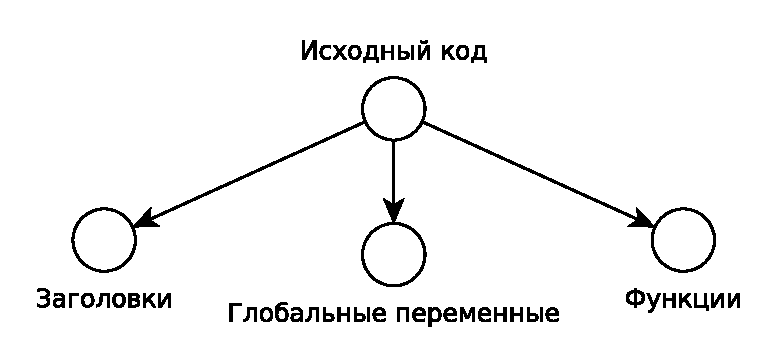
\includegraphics[width=\textwidth]{inc/structure.pdf}
	\caption{Представление структуры исходного кода в виде дерева}
	\label{fig:structure}	
\end{figure}


Каждая часть так же представляется в виде дерева и может иметь вложенную структуру. Например, функция может содержать блок, который имеет следующую структуру:
\begin{itemize}
	\item локальные переменные (тоже самое, что и глобальные, но существуют и доступны только в рамках блока);
	\item информацию о вызываемых функциях, операциях;
	\item контрольный блок: может состоять из контрольного условия или содержать ещё один блок.
\end{itemize}

После построения дерева его можно преобразовать в файл формата \textit{XML}

\noindent\cite{xml} для дальнейшего анализа. Пример структуры файла можно увидеть в листинге \ref{lst:xml-structure}.

\begin{code}
	\captionof{listing}{Эквивалент рисунка \ref{fig:structure}}
	\label{lst:xml-structure}
	\inputminted
	[
	frame=single,
	framerule=0.5pt,
	framesep=20pt,
	fontsize=\small,
	tabsize=4,
	linenos,
	numbersep=5pt,
	xleftmargin=10pt,
	]
	{text}
	{inc/structure.xml}
\end{code}

Далее на основе узлов дерева, с помощью отображений, строятся уникальные последовательности, которые потом будут записаны в матрицу последовательностей. Так, например, для узла заголовков программы будет верно отображение из таблицы \ref{tab:headers}.

\begin{table}[h]
	\begin{center}
		\caption{Матричное отображение узла заголовков.}
		\label{tab:headers}
		\begin{tabular}{|c|c|c|c|}
			\hline
			\bfseries Позиция & $d_{i1}$ & $\dots$ & $d_{in}$ \\
			\hline
			Название заголовка & заголовок$_1$ & $\dots$ & заголовок$_{n}$\\ \hline
		\end{tabular}
	\end{center}
\end{table}

Аналогично для узлов глобальных переменных и функций, где каждому идентификатору присваивается свой уникальный номер. Таким образом для некоторой функции у которой тип возврата $rt_2$, аргументы имеют тип $at_2,at_3,$ $at_{n-k}$, где каждый из типов встречается 2, 3 и $n-k$ раз соответственно, переменные $lt_2,lt_7,lt_k$ и контрольные типы $ct_1,ct_2,ct_{n-k-1}$ можно получить матрицу следующего вида:

\[ \left| 
\begin{array}{c}
	\text{тип возврата}\\
	0~1 ~0~ 0~ 0~ 0~ 0~ 0~ ... ~0~ 0 \\
	0~ 2~ 0~ 0~ 0~ 0~ 3~ 0~ ...~ 0~ 7 \\
	\text{лок. переменные}
\end{array} \right|
\left.\begin{array}{c}
	\text{аргументы}\\
	0~2 ~3~ 0~ 0~ 0~ 0~ 0~0~0~0~0~ ... ~0~ 4 \\
	1~1 ~0~ 0~ 0~ 0~ 0~ 0~0~0~0~0~ ...~ 4~ 0 \\
	\text{контрольные типы}
\end{array}\right|
\] 


Так же на основе \textit{XML} файла строится матрица контрольных последовательностей, где каждой контрольной инструкции функции присваивается свой уникальный номер, чтобы составить уникальную последовательность. Для данной матрицы будет верно отображение из таблицы \ref{tab:control-sequence}

\begin{table}[h]
	\begin{center}
		\caption{Матричное отображение контрольных последовательностей. Значение 99 -- признак того, что для конкретного номера в последовательности нет контрольной инструкции.}
		\label{tab:control-sequence}
		\begin{tabular}{|c|c|c|c|c|c|c|}
			\hline
			\bfseries Контрольная инструкция & $c_1$ & $c_2$ &\dots &$c_1$ & &  \\
			\hline
			Порядок следования & 1 & 2 & $\dots$ & 6 &$\dots$ &$n$ \\ \hline
			Номер & 1 & 2& $\dots$ &1 & $\dots$ & 99\\ \hline
		\end{tabular}
	\end{center}
\end{table}

На последнем этапе преобразований из матрицы последовательностей и матрицы контрольных последовательностью строится интегральная матрица. По каждой строке производится операция суммирования с дальнейшей нормализацией. В конечном итоге каждой строке, которой соответствуют блоки заголовков, глобальных переменных и функций, соответствует нормализованный коэффициент схожести, который находится в диапазоне от 0 до 1. При итоговом подсчёте для каждой строки будет учитываться свой вес $\omega$, так как, блок функций более важен в контексте определения плагиата, чем блок заголовков.

\subsubsection{Анализ абстрактного синтаксического дерева}

Абстрактное синтаксическое дерево (англ. Abstract Syntax Tree (AST\cite{AST})) -- представление абстрактной синтаксической структуры в виде дерева, в котором внутренние вершины сопоставлены (помечены) с операторами языка программирования, а листья -- с соответствующими операндами. АСД широко используются инфраструктурами компиляторов в качестве промежуточного представления (ПП) исходного кода. Ниже рассмотрим алгоритм, основанный на сравнении двух АСД, полученных с помощью утилиты \textit{Clang}\cite{clang} фреймворка \textit{LLVM}\cite{llvm}.

Так как исходный код можно представить в виде АСД, изменения можно получить используя разницу между деревьями. Такой подход перспективен потому, что точная информация о каждом изменении присутствует в АСД. Выделяют три основных типа узлов:
\begin{enumerate}
	\item Declarations -- объявления;
	\item Statements -- инструкции;
	\item Types -- типы.
\end{enumerate}

Например, АСД для выражения $a=b\times c +d\div e$ может быть представлено, как на рисунке \ref{fig:ast-ex}.

\clearpage

\begin{figure}[h!btp]
	\centering
	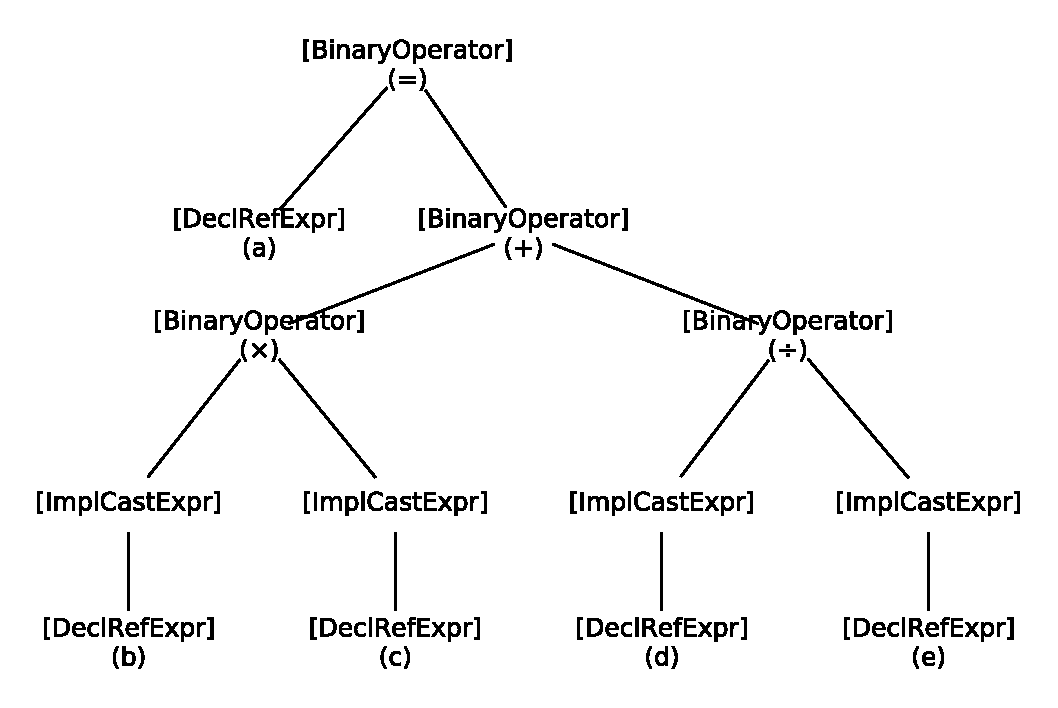
\includegraphics[width=\textwidth]{inc/ast-ex.pdf}
	\caption{Представление структуры исходного кода в виде дерева}
	\label{fig:ast-ex}	
\end{figure}

Рассмотрим два алгоритма, использующих в своей основе АСД: сравнение деревьев, с помощью строковых ядер\cite{string-kernel}\cite{ast-aproach} и классификация изменений в структуре дерева\cite{ast-op-values}.

Для первого метода нужно представить дерево в виде строки, таким образом, в результате прямого обхода, из дерева на рисунке \ref{fig:ast-ex} получим следующую строку: 
$
\texttt{[BinaryOperator]}_1\texttt{[DeclRefExpr]}_1\texttt{[LEVEL\_UP]}_1...\texttt{[LEVEL\_UP]}_5
$

Для оптимизации занимаемого пространства применяются следующие операции:
\begin{itemize}
	\item последовательность одинаковых узлов заменяется одним с суммированием весов:
	\item [] $
	\begin{array}{c}
			\texttt{[BinaryOperator]}_1\texttt{[BinaryOperator]}_1\texttt{[BinaryOperator]}_1\\
			\downarrow\\
			\texttt{[BinaryOperator]}_3
	\end{array}$

	\item удаляются узлы показывающие вызов функций и преобразования типов. Количество удалённых узлов суммируется с весом потомка:
	\item [] $
	\begin{array}{c}
		\texttt{[CStyleCastExpr]}_1\texttt{[CallExpr]}_1\texttt{[ImplicitCallExpr]}_1\texttt{[DeclRefExpr]}_1\\
		\downarrow\\
		\texttt{[DeclRefExpr]}_4
	\end{array}$

	\item удаляются узлы между $\texttt{[DectStmt]}$ и $\texttt{[LEVEL\_UP]}$. Количество удалённых узлов суммируется с весом родителя:
	\item [] $
	\begin{array}{c}
		\texttt{[DeclStmt]}_1\texttt{[VarDecl]}_1\texttt{[DeclRefExpr]}_1\texttt{[LEVEL\_UP]}_4\\
		\downarrow\\
		\texttt{[DeclStmt]}_3\texttt{[LEVEL\_UP]}_4
	\end{array}$

	\item идентичные узлы суммируются между собой:
	\item [] $
	\begin{array}{c}
		\texttt{[IntegerLiteral]}_2\texttt{[LEVEL\_UP]}_5\\
		\texttt{[IntegerLiteral]}_4\texttt{[LEVEL\_UP]}_2\\
		\downarrow\\
		\texttt{[IntegerLiteral]}_6\texttt{[LEVEL\_UP]}_7
	\end{array}$
\end{itemize}

Полученные строки анализируются на вхождение идентичных блоков, при поиске вхождений учитывается полное соответствие последовательности и разница в весах частей. Таким образом можно находить процент различия отдельно взятых последовательностей. Результатом является нормализованный коэффициент схожести, который находится в диапазоне от 0 до 1.

Для второго метода можно сказать, что из одного дерева, можно получить другое путём применения некоторых операций. Определим четыре действия\cite{ast-op-values}:
\begin{enumerate}
	\item вставка узла в дерево: $INS((l,v),y,k)$, где $l$ -- название узла, $v$ -- его значение, $k$ -- порядковый номер потомка, $y$ -- узел родителя;
	\item удаление узла из дерева: $DEL(x)$, где $x$ потомок некоторого узла $p(x)$;
	\item перемещение узла: $MOV(x,y,k)$, где $x$ -- перемещаемый узел, $k$ -- новый порядковый номер потомка, $y$ -- новый родитель $x$;
	\item обновление (изменение) узла: $UPD(x, v)$, где $x$ - обновляемый (изменяемый) узел, $v$ -- новое значение при условии $v_{old}\neq v_{new}$.
\end{enumerate}

Каждое действие имеет своё определённое влияние в контексте использования, например, изменение условия в условном блоке оказывает больше влияния, чем изменение названия переменной. Удаление какой-либо функциональности является <<критическим>> изменением. 

Текущая реализация -- \textit{ChangeDistiller}\cite{change-distiller}. Алгоритм строит ещё одно дерево на основе АСД, обрабатывает его находя разницу между узлами и индексирует возможный список операций, применённый к дереву. Различия между узлами находятся с помощью редакционного расстояния\cite{levenshtein}. Данный подход является менее эффективным, в сравнении с предыдущим -- преимущественно точен для объектно-ориентированных языков и требует дополнительных вычислений.

\clearpage

\specsection{ЗАКЛЮЧЕНИЕ}

Готовые решения в области систем управления обучением, зачастую являясь системами общего назначения, предоставляют ограниченный набор функционала без возможности его расширения. Некоторые системы предоставляются <<как есть>> даже без возможности обращения в поддержку. Сравнение рассмотренных систем управления обучением можно увидеть в таблице \ref{tab:res}. Обозначения:
\begin{itemize}
	\item Б -- бесплатное распространение;
	\item П -- платное распространение;
	\item Ч -- частично удовлетворяет критерию.
\end{itemize}

\begin{table}[h]
    \begin{center}
        \caption{Анализ систем управления обучением.}
        \label{tab:res}
        \begin{tabular}{|c|c|c|c|}
            \hline
            \bfseries Критерий &\bfseries Moodle & \bfseries Canvas & \bfseries Algorithmi \\
            \hline
            распространение & Б/П & Б/П & Б\\ \hline
            поддержка & П & П & - \\ \hline
            возможность расширения & Ч & - & - \\ \hline
            интеграция сторонних систем & Ч & -  & -\\ \hline
            антиплагиат & - & - & + \\ \hline
            создание учебного материала & + & + & - \\ \hline
			организация курса & + & + & - \\ \hline
			кроссплатформенность & Ч & + & Ч \\ \hline
        \end{tabular}
    \end{center}
\end{table}

В отличие от алгоритмов поиска заимствования в литературе, выбор подхода для определения заимствований в программировании является очень существенным \cite{antiplagiat-xml}. Программная или графическая реализация может претерпевать до шести уровней модификаций, чтобы обойти антиплагиат. Ознакомиться с предполагаемыми уровнями модификаций можно на рисунке \ref{fig:anti-levels}.

\begin{figure}[h!btp]
	\centering
	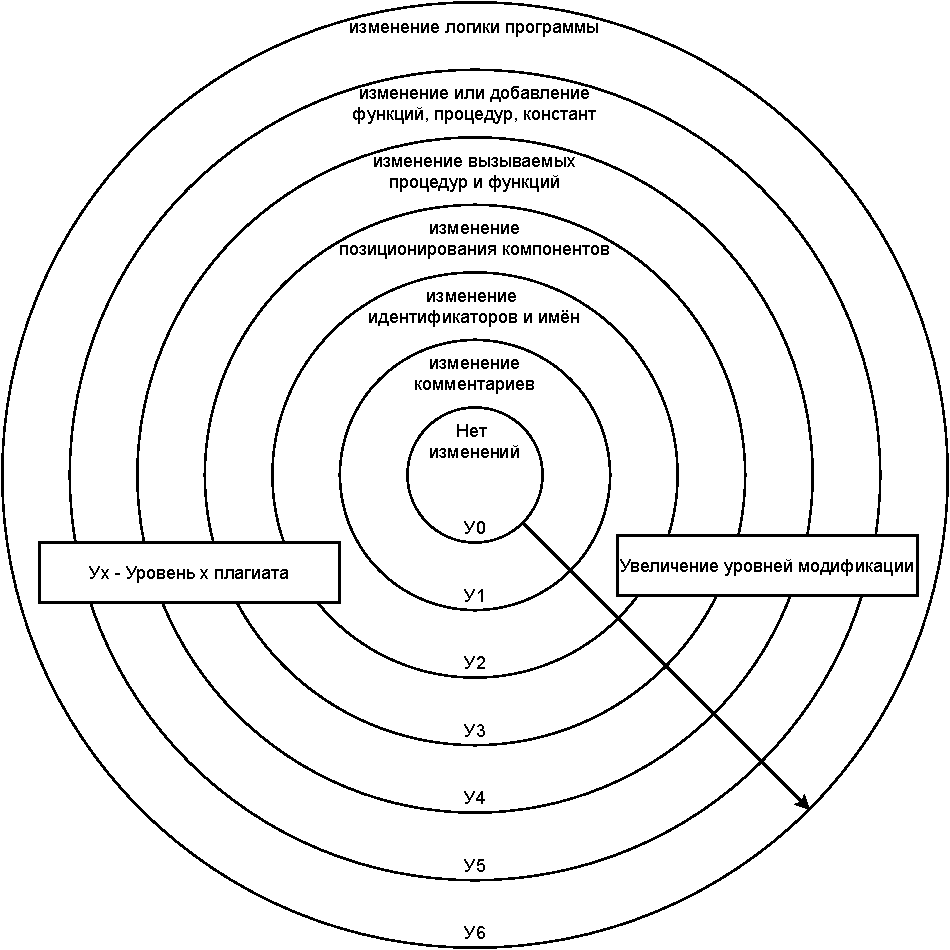
\includegraphics[width=\textwidth]{inc/levels.pdf}
	\caption{Спектр модификаций}
	\label{fig:anti-levels}	
\end{figure}

\clearpage

\specsection{СПИСОК ИСПОЛЬЗОВАННЫХ ИСТОЧНИКОВ}

\begingroup
\renewcommand{\section}[2]{}
\bibliographystyle{utf8gost705u}
\bibliography{bibliography}   
\endgroup

\end{document}
